\section{Use Cases: Personenverwaltung (5123101)}
	Im folgenden werden die Use Cases zur Personenverwaltung beschrieben. Darüber hinaus wird der Aufbau der zugehörigen Datenbanktabellen beschrieben.

\begin{table}[h]
\centering
\renewcommand{\arraystretch}{1.4}
\begin{tabularx}{\textwidth}{|p{4cm}|X|}
\hline
\textbf{Titel} & \textbf{Patientenverwaltung} \\
\hline
\textbf{Kontext} & 
Damit ein Patient stationär aufgenommen werden kann, muss dieser zuerst als Person in der Krankenhaus Datenbank angelegt werden und eine Zuordnung als Patient erfolgen \\
\hline
\textbf{Beschreibung} & 
Der Use Case beschreibt die Erfassung und Pflege aller personenbezogenen Daten. 
Bei der Aufnahme eines neuen Patienten werden zunächst die allgemeinen Stammdaten 
in der Tabelle \texttt{person} gespeichert. Anschließend erfolgt die Anlage eines 
zugehörigen Eintrags in der Tabelle \texttt{patient}, wodurch die Person fachlich 
als Patient klassifiziert wird. Bestehende Daten können jederzeit aktualisiert werden, 
wobei Änderungen an allgemeinen Informationen in \texttt{person} und patientenspezifische 
Anpassungen in \texttt{patient} erfolgen. \\
\hline
\end{tabularx}
\caption{Use Case: Patientenverwaltung}
\label{tab:usecase_patient}
\end{table}

\newpage

\begin{table}[h]
\centering
\renewcommand{\arraystretch}{1.4}
\begin{tabularx}{\textwidth}{|p{4cm}|X|}
\hline
\textbf{Titel} & \textbf{Mitarbeiterverwaltung} \\
\hline
\textbf{Kontext} & 
Anlegen und verwalten eines Mitarbeiters durch die Administration \\
\hline
\textbf{Beschreibung} & 
Der Use Case umfasst die Erfassung und Pflege aller Mitarbeitenden im Krankenhaus. 
Zunächst werden die allgemeinen Personendaten in der Tabelle \texttt{person} angelegt. 
Darauf aufbauend wird ein Eintrag in \texttt{employee} erstellt, wodurch die Person 
als Mitarbeitender geführt wird. Ein Mitarbeiter erhält hierbei noch die Zuordnung zu seinem Fachbereich mit einer Referenz auf einen Eintrag in der Tabelle \texttt{departement} in dem er arbeitet. Daraufhin erfolgt eine Spezialisierung als Arzt oder 
Pflegekraft durch zusätzliche Einträge in den Tabellen \texttt{doctor} bzw. 
\texttt{nurses}. Änderungen bestehender Daten werden je nach Art der Information 
in den entsprechenden Tabellen vorgenommen. \\
\hline
\end{tabularx}
\caption{Use Case: Mitarbeiterverwaltung}
\label{tab:usecase_employee}
\end{table}

\subsection*{Datenverwaltung}
Bei der Datenverwaltung ist eine Besonderheit, dass die Daten zu allen Personen gesammelt in der Tabelle \texttt{person} gespeichert werden. 
Darüber hinaus werden in den Tabellen \texttt{patient} und \texttt{employee} nur die Referenzen zum Eintrag in \texttt{person} angeführt. Dies hat den Vorteil, dass einige Spalten nicht doppelt aufgeführt werden müssen. Um mit diesem Vorgehen eine eindeutige Zuordung zu gewährleisten, besteht jeweils zwischen \textit{person} und \textit{patient} und \textit{person} und \textit{employee} eine 1:1 Beziehung.
Die Tabelle \textit{employee} wird zudem in \texttt{nurses} und \texttt{doctors} aufgeteilt.
Desweitern werden die personenbezogenen Daten in der Tabelle \texttt{person} verschlüsselt abgespeichert um die Sicherheit der Daten zu gewährleisten. Im nachfolgenden ist eine Graphik, die den Aufbau der benötigen Tabellen veranschaulicht. 

\begin{figure}[h]
    \centering
    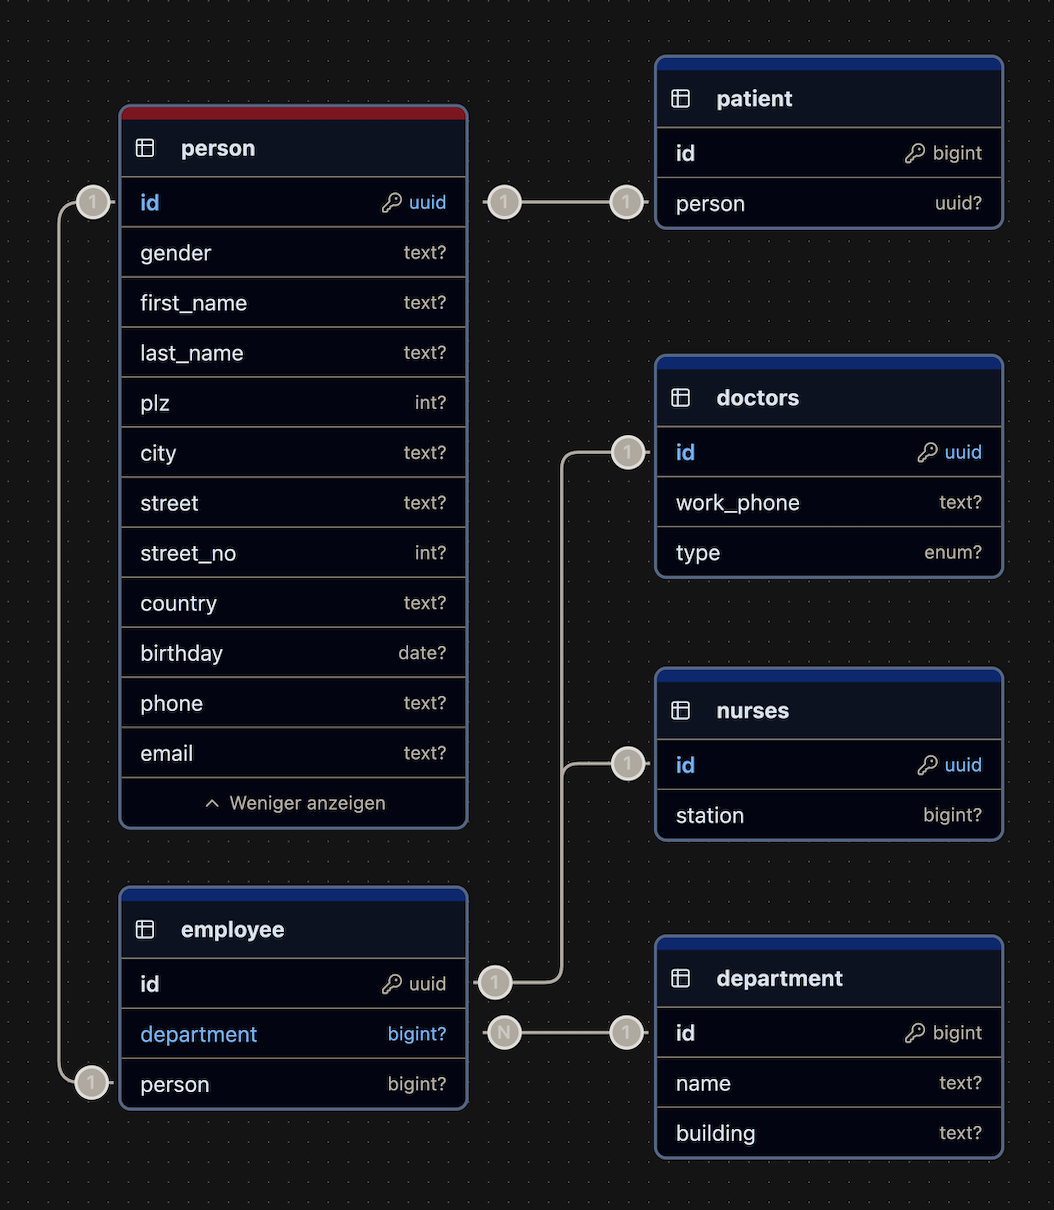
\includegraphics[width=0.8\textwidth]{Bereiche_Datenmodell/Personenverwaltung.png}
    \caption{Personenverwaltung}
\end{figure}

